\chapter*{Lecture 11}
\begin{recall}{}{}
\begin{itemize}
\item Applications of ODE: falling objects
\item Intro to circuits
\end{itemize}
\end{recall}




\begin{exmp}{Current in a LR circuit:}\\
A simple resistor-inductor circuit as shown below. At $t=0$, the knife switch is closed and current, $I(t)$, flows through the circuit due to the applied voltage $E_0$. Find the differential equation for $I(t)$. $L=0.1$ henry and $R=100$ $\Omega$ .
\begin{enumerate}
\item {Problem Statement}\\
\begin{minipage}{0.6 \textwidth}
\begin{itemize}
\item Pictorial representation
\item Variables: $t$, $I(t)$
\item Parameters: $L$, $R$, $E_0$
\end{itemize}
\end{minipage}
\begin{minipage}{0.25 \textwidth}
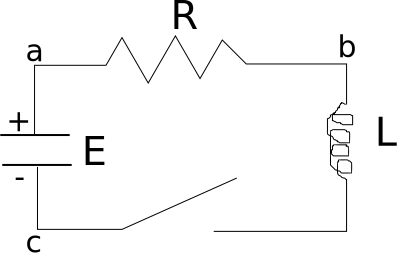
\includegraphics[width=\textwidth]{figs/LRcircuit.pdf} 
\end{minipage}
\item {Mathematical model}\\
\begin{itemize}
\item Physical law: Kirchhoff's voltage law
\item Mathematical expression: 
\begin{equation*}
\sum  \Delta E = \underbrace{(E_a-E_b)}_{\text{resistor}} +  \underbrace{(E_b-E_c)}_{\text{inductor}}+ \underbrace{(E_c-E_a)}_{\text{applied voltage}}=0
\end{equation*}
\item Physical law into an ODE:
\begin{equation*}
(E_a-E_b) = RI(t)\qquad (E_b-E_c)=L\frac{dI(t)}{dt}\qquad (E_a-E_a)=-E_0
\end{equation*}
\begin{equation*}
RI(t)+L\frac{dI(t)}{dt}-E_0=0 \qquad or \qquad \frac{dI(t)}{dt}+\frac{R}{L}I(t)=\frac{E_0}{L}
\end{equation*}
with the IC: $t=0$, $I(t)=0$.
\end{itemize}
\item {solve the ODE}\\
Method: First-order ODE formula\\
\begin{equation*}
 \frac{dI(t)}{dt}+\underbrace{\frac{R}{L}}_{p(t)}I(t)=\underbrace{\frac{E_0}{L}}_{q(t)}
\end{equation*}
Find an integrating factor such that:
\begin{equation*}
 U=e^{\int p(t) dt}=e^{\int \frac{R}{L} dt}=e^{\frac{R}{L}t}
 \end{equation*}
The current can be computed as:
\begin{equation*}
 I(t)=\frac{1}{e^{\int p(t) dt}}\left[\int q(t)e^{\int p(t) dt} dt+c_1\right]
 \end{equation*}\par


The general solution is:
\begin{equation*}
 \boxed{I(t)=\frac{E_0}{R}+c_1e^{-\frac{R}{L}t}}
\end{equation*}
Apply the IC: $t(0)=0$, $I(t)=0$

\begin{equation*}
0=\frac{E_0}{R}+c_1\qquad or \qquad c_1=-\frac{E_0}{R}
\end{equation*}
The final (particular) solution is:
\begin{equation*}
 \boxed{I(t)=\frac{E_0}{R}\left(1-e^{-\frac{R}{L}t}\right)}
\end{equation*}

\item Applications:\\
Compute the time constant when $L=0.1$ henry and $R=100 \Omega$\\ 
The time constant is defined as the time it takes the system to reach: $1-1/e\approx 63.2\%$.\\
The maximum current is defined as $t\rightarrow\infty$:
\begin{equation*}
I(t)=\frac{E_0}{R}\left(1-\underbrace{e^{-\frac{R}{L}t}}_0\right)=\frac{E_0}{R}
\end{equation*}
Therefore, we need to find the time at which $I(t)=0.632 \frac{E_0}{R}$.
Simple algebraic manipulations lead us to: $t=L/R=0.001$
\end{enumerate}
\end{exmp}
\begin{center}
\noindent\rule{4cm}{0.4pt}
\end{center}




\subsection{Heating and cooling}


\begin{testv}{}{}
What can affect the temperature of a given system? For simplicity, we consider the heating and cooling of a building:
\begin{itemize}
\item Heat produced by people inside the building (source: $S_{people}$)
\item Heating or cooling supplied by a furnace or air conditioner (source/sink: $S_{source}$)
\item Outside temperature (boundaries)
\end{itemize}
Newton's law of cooling states that the rate of change in temperature $T(t)$ is proportional to the difference between the outside temperature $M(t)$ and the inside temperature $T(t)$. In other words:
\begin{equation*}
K\left(M(t)-T(t)\right)
\end{equation*}
When the temperature outside is greater $(M(t)-T(t))>0$, the temperature inside will increase; if the temperature outside is lower, the temperature inside will decrease.

The governing equation for these problems are:
\begin{equation*}
\frac{dT(t)}{dt}=K\left[M(t)-T(t)\right] + S_{people}+S_{source}
\end{equation*}

As this equation is linear, we can solve it following the method of linear equations (section 2.3).

\begin{equation*}
\frac{dT(t)}{dt}+P T(t)=Q
\end{equation*}
where $P=K$ and $Q=KM+S_{people}+S_{source}$
\end{testv}

\begin{center}
\noindent\rule{4cm}{0.4pt}
\end{center}


\begin{exmp}{Jello:}\\
Suppose you prepare a huge amount of Jello. To fully dissolve the sugars, the package suggests that you mix the content to a given amount of boiling water (at 100$^\circ$ C). For the Jello to harden, it needs to cool down rapidly (previous experience with watery Jello after adding ice-cubes need not be repeated). To cool the Jello down rapidly, you set the pot in a sink with running cold water (water is at 5$^\circ$ C). The temperature of the Jello drops to 60$^\circ$ C) after 10 minutes (HUGE pot of Jello). How long do you need to cool the Jello it until you can put it in the fridge at 20$^\circ$ C? (assume that it is perfectly mixed)\\

\textbf{Solution:}\\
\begin{enumerate}
\item {Problem Statement}\\
\begin{minipage}{0.6 \textwidth}
\begin{itemize}
\item Pictorial representation
\item Variables: $t$, $T(t)$
\item Parameters: $T_{ambient}$
\end{itemize}
\end{minipage}
\begin{minipage}{0.25 \textwidth}
\includegraphics[width=\textwidth]{figs/jello.jpg} 
\end{minipage}
\item {Mathematical model}\\
\begin{itemize}
\item Physical law: Newton's cooling law
\item Mathematical expression: 
\begin{equation*}
\frac{dT}{dt}=K\left[T_{ambient}-T(t)\right]
\end{equation*}
Typically $K$ is positive. Does this equation make sense? Sould $dT/dt$ be positive/negative?\\

The problem also states the initial condition:  $t=0$, $T(t=0)=100^\circ C$.
\end{itemize}

\item {solve the ODE}\\
Method: First-order linear ODE formula\\
\begin{equation*}
 \frac{dT(t)}{dt}+\underbrace{K}_{p}T(t)=\underbrace{K T_{ambient}}_{q}
\end{equation*}

Find an integrating factor such that:
\begin{equation*}
 U=e^{\int p(t) dt}=e^{\int K dt}=e^{Kt}
 \end{equation*}
Multiply both sides by $U$ and integrate:
\begin{equation*}
 T(t)=\frac{1}{e^{\int p(t) dt}}\left[\int q(t)e^{\int p(t) dt} dt+c_1\right]
 \end{equation*}
\begin{equation*}
 T(t)=\frac{1}{e^{Kt}}\left[K T_{ambient} \int {e^{Kt}} dt+c_1\right]=\left[  T_{ambient} +\frac{c_1}{e^{Kt}}\right]
 \end{equation*}

The general solution is:
\begin{equation*}
 \boxed{T(t)=T_{ambient} +c_1 e^{-Kt}}
\end{equation*}
Apply the IC: $t=0$, $T(t)=100$ ($T_{ambient}=5^\circ C$)


\begin{equation*}
100=5 +c_1  \qquad or \qquad c_1=95
\end{equation*}
The particular solution is:
\begin{equation*}
 \boxed{T(t)=T_{ambient} +95 e^{-Kt}}
\end{equation*}

\item Applications:\\
How do we define the time needed to cool down the Jello? We need to estimate $K$!\\
We know that at $t=10$  min (600 s), we have a temperature of $T=60$, therefore:

\begin{equation*}
 60=5 +95 e^{-K(600)}
\end{equation*}
or:

\begin{equation*}
 \ln{\frac{55}{95}} = -K(600)
\end{equation*}
The value of $K=9.1904 E-4$.\\
Now we can compute the time necessary to bring the Jello down to 20 deg.
\begin{equation*}
 20=5 +95 e^{- 9.1904 E-4 t}
\end{equation*}
we find $t\approx 2000$ s (about 33 min).\\
\end{enumerate}


\end{exmp}
\begin{center}
\noindent\rule{4cm}{0.4pt}
\end{center}
